%%%%%%%%%%%%%%%%%%%%%%%%%%%%%%%%%  Dual-phase
\subsection{Introduction}
\label{sec:fddp-slow-cryo-intro}

% RC:
% - Clarity could be increased by making the document more consistent about what systems are included in the \dword{cisc} scope. Figure 1.1 contains several items that are not mentioned elsewhere in the document: "Instrumentation Feed-throughs," "Feedthrough contamination studies," and "Instrumentation Precision Studies."
% - Firmware and racks are mentioned in the introduction but not elaborated on much later in the document or included in Fig. 1.1.
% - E-field simulations are mentioned in the Introduction and Interface sections but not described in the main body (Sec. 1.2 and 1.3).
% - A clear statement in words (or as a boundary on Fig. 1.1) of the exact border between DUNE and LBNF would be very helpful. One particularly unclear point is whether feed-throughs are the responsibility of DUNE or LBNF.


% identical for SP and DP (updated by Anne along with SP)
The \dword{cisc} system provides 
comprehensive monitoring for all \dword{detmodule} components as well as for the \lar quality and behavior, both being crucial
to guarantee high-quality of the data. Beyond passive monitoring, \dword{cisc} also provides a control system for some of the detector components. 
The structure of the \dword{cisc} consortium is quite complex. A subsystem chart
for the \dword{cisc} system is shown in Figure~\ref{fig:sp-slow-cryo-subsys}. 

\begin{dunefigure}[CISC subsystems]{fig:sp-slow-cryo-subsys}
{\dword{cisc} subsystem chart}
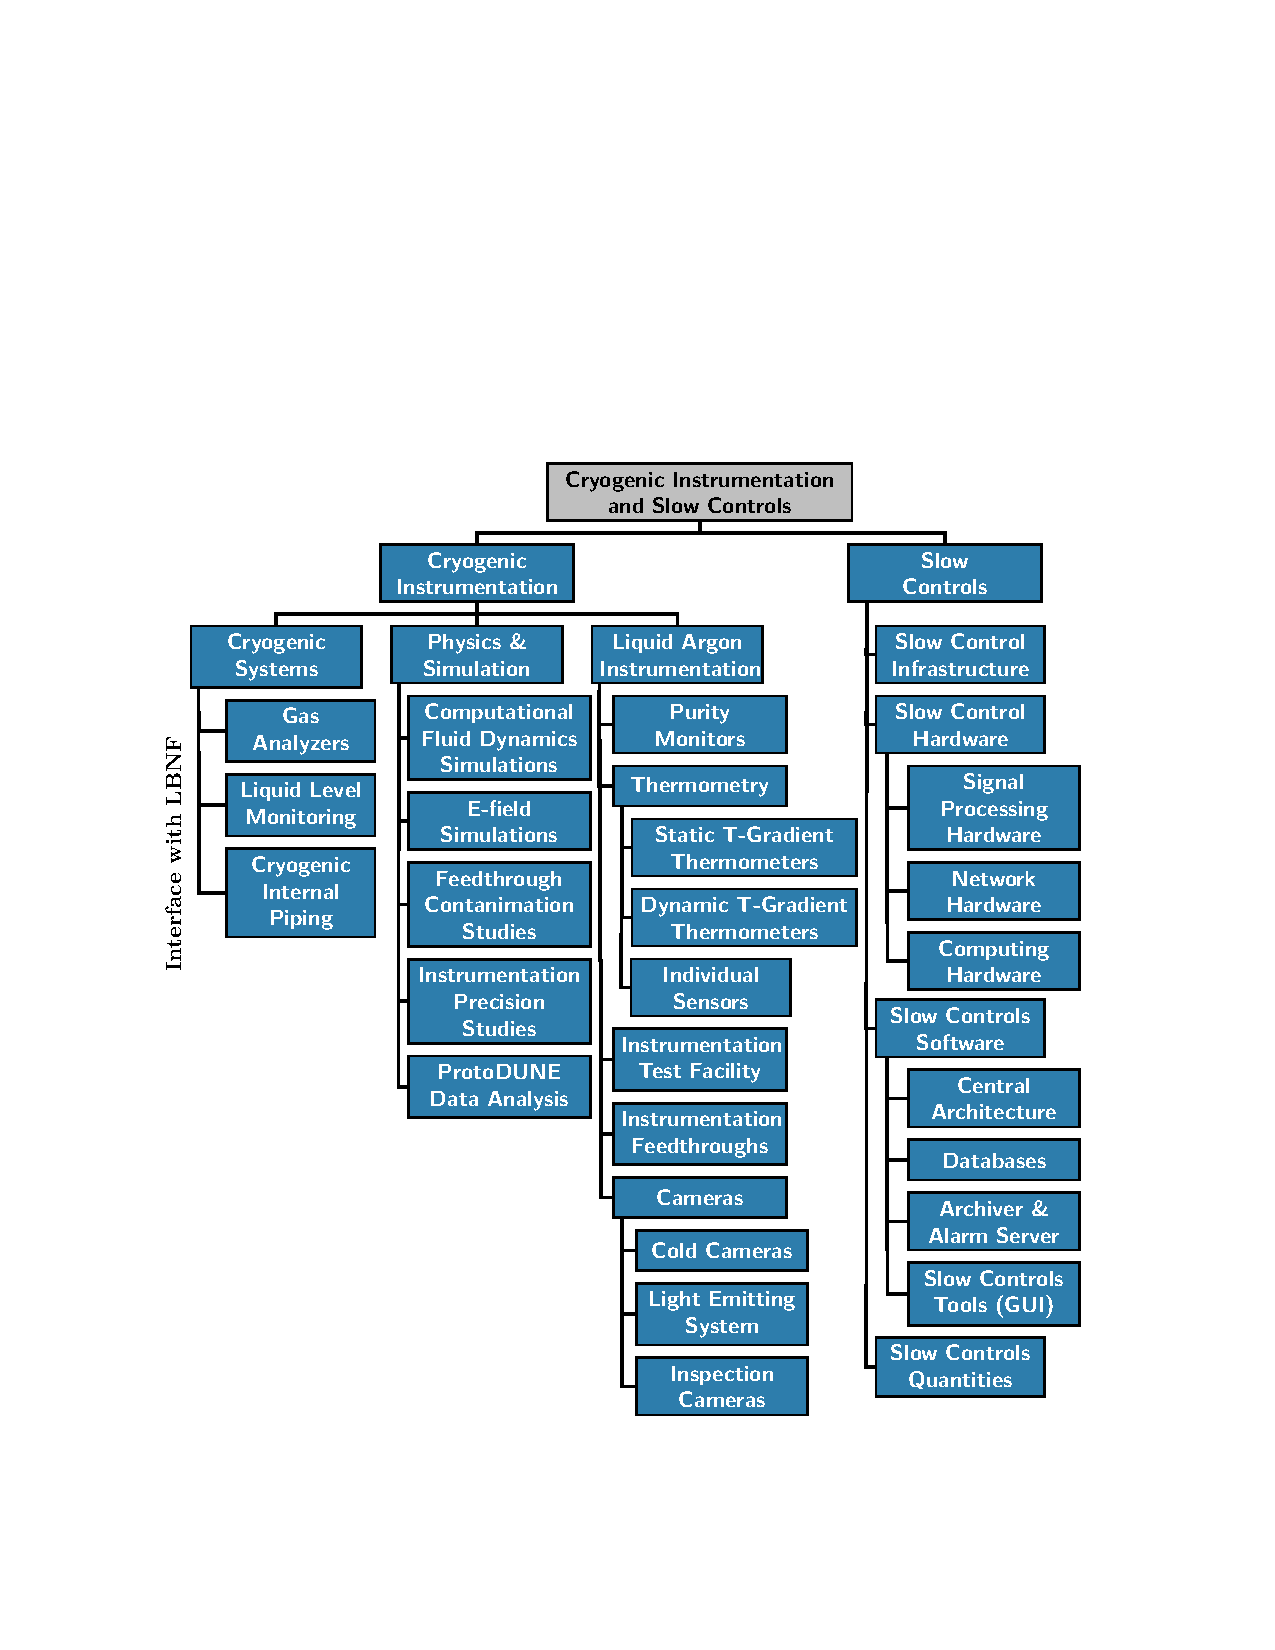
\includegraphics[width=0.5\textwidth,trim=20mm 30mm 30mm 70mm,clip]{cisc_subsys-new}  %{cisc_subsys}  update organizational chart for consistency - ddm
\end{dunefigure}

Two main branches can be distinguished: cryogenic instrumentation and slow controls. The former includes a set of devices 
to monitor the quality and behavior of the \lar volume in the cryostat interior, ensuring the correct functioning of
the full cryogenics system and the suitability of the \dword{lar} for good quality physics data. Those devices are 
purity monitors, temperature monitors, gas analyzers, \lar level monitors, and cameras with their associated
light emitting system.

Cryogenic instrumentation also requires significant physics and
simulation work such as \efield simulations and cryogenics modeling
studies using \dfirst{cfd}. \efield simulations
are required to identify desirable locations for instrumentation
devices in the cryostat so that they are not in regions of high \efield and
that their presence do not induce large field distortions. \dshort{cfd}
% AC. What do we mean by distorsions here ?
% Alternative: ``that their designs do not induce high electric fields and risk of dielectric breakdown. ``
simulations are needed to understand the expected temperature,
impurity and velocity flow distributions and guide the placement and
distribution of instrumentation devices inside the cryostat.


From the organizational point of view
cryogenic instrumentation has been divided into three main parts: (1) cryogenics systems, which includes all components directly related to the external cryogenics system as
liquid level monitoring, gas analyzers and internal cryogenic piping, all having substantial interfaces with LBNF; (2) \lar  instrumentation, which includes all
other instrumentation devices; and (3) physics and simulation.


The second branch of \dword{cisc} is the slow controls system, in charge of monitoring and control most detector elements, as power supplies, electronics, racks, instrumentation devices,
calibration devices, etc. It includes four main components: hardware, infrastructure,
software, and firmware. The slow controls hardware and infrastructure consists of
networking hardware, signal processing hardware, computing hardware, and relevant
rack infrastructure. The slow controls software and firmware is needed for
signal processing, alarms, archiving, and control room displays.

Two other systems have been included by the DUNE management as part of the \dword{cisc} consortium,
a test facility for the instrumentation devices and the cryogenic piping inside the cryostat.
Those are included inside the cryogenic instrumentation branch.

%The instrumentation work related to gas analyzers, liquid level
%monitors and internal cryogenic piping has significant
%interface with LBNF and will be coordinated between DUNE and LBNF.


%%%%%%%%%%%%%%%%%%%%%%%%%%%%%%%%%%%%%
\subsection{Design Considerations}
\label{sec:fddp-slow-cryo-des-consid}

% specific to DP

For all \lar instrumentation devices, \dword{pddp} designs are
considered as the baseline, and requirements for most design
parameters are extrapolated from \dword{protodune}. Hence a critical step for
the \dword{cisc} consortium is to analyze data from \dword{protodune} when available
to validate the instrumentation designs and understand their
performance. For example, a crucial design parameter, which should be evaluated in \dword{protodune},
is the maximum noise level induced by instrumentation devices on the readout electronics that can be tolerated to avoid confusing event reconstruction. 

Some of the common design considerations for
instrumentation devices include stability, reliability and longevity
such that the devices can survive for a period of at least \dunelifetime{}.  Since it is uncommon for any device
to have such a long lifetime, provisions are made in the overall
design to allow replacement of devices where possible.

As for any other element inside the cryostat, 
the electric field on the instrumentation devices is 
required to be less than \SI{30}{kV\per\cm},
so that the risk of dielectric breakdown in \dword{lar} is minimized.
This requirement imposes stringent constraints on the location and mechanical 
design of some devices. Electrostatic simulations  
will be performed to compute the expected field on the boundaries of 
instrumentation devices and to design the appropriate \efield shielding
in the case the electric field approaches the limit. 

Another common consideration for all instrumentation devices is their support structure
design, which is expected to be substantially different from the one used in \dword{protodune}.

For slow controls, the system needs to be designed such that it is 
robust enough to support a large number of monitored variables, a broad range of
monitoring and archiving rates, and has the capability of interfacing 
with a large number of systems to establish two-way communication for
control and monitoring. Table \ref{tab:dp-cisc-requirements} shows
some of the important \dword{cisc} system design requirements.

There are several aspects specific to the \dual design impacting the \dword{cisc} system design requirements:
\begin{itemize}
\item At the level of the cryogenic instrumentation, additional care is needed in order to monitor the gas phase above the liquid level. The temperature and the pressure of the gas phase affect the gas density, and consequently, the \dword{lem} gain calibration. The gas pressure must be accurately monitored. In proximity to the liquid surface the temperature gradient of the gas %has to be 
is measured with an array of temperature probes with a vertical pitch of about \SI{1}{cm}. Each \dword{crp} is also equipped with \num{36} thermometers to sample the temperature across its structure.

\item The \dword{crp}-specific instrumentation also includes: 

%%%%
\begin{itemize}
\item the pulsing system for charge injection in the anode strips,
\item the precision level meters implemented only on the \dwords{crp} located at the cryostat borders, and 
\item the measurement of the \dword{lem}-grid capacitance allowing to know \fixme{which provides} the position of the \dword{crp} with respect to the liquid level for all \dwords{crp}, \fixme{what makes the measurement?}
\item the control of the stepping motors, \fixme{control mechanism?} which allows positioning each \dword{crp} parallel to the liquid level (keeping the extraction grid immersed in the liquid and the \dwords{lem} in the gas phase).
\end{itemize}
%%%%%%

%\item The slow control system should provide the generation and control of \dword{hv} biasing of \dword{lem} and of the extraction grid respectively at a maximum voltage of  -5 kV/channels for the LEM (41 channels/CRP) biasing and -10kV/channel for the grid biasing (1 channel/CRP);
\item The slow control system generates and controls the \dword{hv} for biasing the \dwords{lem} (\num{41} channels/\dword{crp}) and the extraction grid  (\num{1} channel/\dword{crp}), at maximum voltages of  \SI{-5}{kV/channel} and \SI{-10}{kV/channel}, respectively;
\item The requirements related to the \dword{pds} include the generation and control of \dword{hv} biasing for the \dwords{pmt} (up to \SI{-3}{kV}) and the control of the calibration of the  \dwords{pmt},  performed with a  light distribution system with a common light source and a network of optical fibers;
\item The \dword{fe} electronics requires the control of the \dword{utca} crates, the control of the  analog \dword{fe} cards, the control of the \dword{lv} and of the charge injection system connected to the pre-amplifiers mounted on the \dword{fe} cards;
%\item The \dual design also enables surveying of the \dword{crp} alignment by surveying from the cryostat roof the position of reference points connected to the \dword{crp} suspension system. This aspect needs as well to be integrated in the alignment scheme;
\item The \dual design also enables surveying from the cryostat roof the position of reference points connected to the \dword{crp} suspension system, to ensure proper \dword{crp} alignment. This aspect needs as well to be integrated in the alignment scheme. \fixme{IS integrated?}
\end{itemize}
%A full list of
% requirements for design parameters can be found in DUNE Doc-DB 6440.



\begin{dunetable}
[Important design requirements on the DP CISC system design]
{p{0.22\textwidth}p{0.17\textwidth}p{0.32\textwidth}p{0.19\textwidth}}
{tab:dp-cisc-requirements}
{Important design requirements on the dual phase \dword{cisc} system design}   
Design Parameter
 & Requirement
 & Motivation
 & Comment \\ \toprowrule
Electron lifetime measurement precision
 & $<\SI{1.4}{\%}$ at \SI{3}{ms}
 & Per DUNE-FD Task Force\,\cite{fdtf-final-report}, needed to keep the bias on the charge readout in the \dshort{tpc} to below \SI{0.5}{\%} at \SI{3}{ms}
 & Purity monitors do not directly sample \dshort{tpc}: see Section~\ref{sec:fdgen-slow-cryo-purity-mon}
\\  \colhline
Thermometer precision
 & $<\SI{5}{mK}$
& Driven by \dshort{cfd} simulation validation; based on \dword{pdsp} design
& Expected \dword{protodune} performance \SI{2}{mK}
\\ \colhline
Pressure meters precision (\dual)
 & $<1mbar$
& To measure the pressure (density) of the gas phase; based on \dword{pddp} design
&  \dword{wa105} / \dword{pddp} design $<\SI{1}{mbar}$
\\ \colhline
Thermometer density
 & \(>2/\si{m}\) (vert.), \(\sim\)~\SI{0.2}{m} (horiz.)
 & Driven by \dshort{cfd} simulation.
 & Achieved by design. 
\\ \colhline
Thermometer density gas phase (\dual)
 & \(>1/\si{cm}\) (vert.), \(\sim\)~\SI{1}{m} (horiz.)
 & Vertical array of thermometers with finer pitch close to the liquid level to measure the temperature gradient in the gas phase.
 & Achieved by design. 
\\ \colhline
Thermometer density \dword{crp} structure (\dual)
 & 36 thermometers on each \dword{crp}
 & Monitoring the temperature across the \dword{crp}  structure.
 & Achieved by design. 
\\ \colhline
% Liquid level meters precision (SP)
%  & \SI{0.1}{\%} over \SI{14}{m}
% & Standard sensitivity; will use two level meters for redundancy
% & \dword{protodune} design
% \\  \colhline
Liquid level meters precision (\dual)
 & \(<\SI{1}{mm}\)
&  Maintain constant \dword{crp} alignment with respect to the liquid surface
& \dword{wa105} / \dword{pddp} design \SI{0.1}{mm}
\\  \colhline
 Cameras
 & \multicolumn{3}{p{0.64\textwidth}}{--- multiple requirements imposed by interfaces: see Table~\ref{tab:fdgen-cameras-req} ---}
 \\ \colhline
Cryogenic Instrumentation Test Facility cryostat volumes
 & 0.5 to \SI{3}{m^3}
& Based on filling costs and turn around times
& Under design
\\  \colhline
 Max.\ E-field on instrumentation devices
 & \(<\SI{30}{kV/cm}\)
 & The mechanical design of the system should be such that \efield is below this value, 
 to minimize the risk of dielectric breakdown in \dword{lar}
 & \dword{protodune} designs based on electrostatic simulations
\\ \colhline
 Noise introduced into readout electronics
 & Below significant levels
 & Keep readout electronics free from external noise, which confuses event reconstruction
 & To be evaluated at \dword{protodune}
\\ \colhline
Total no.\ of variables
 & \numrange{50}{100}\si{k}
& Expected number based on scaling past experiments; requires robust base software model that can handle large no. of variables.
& Achievable in existing control systems; DUNE choice in progress.
\\  \colhline
Max.\ archiving rate per channel
 & \SI{1}{Hz} (burst), \SI{1}{\per\minute} (avg.)
& Based on expected rapidity of interesting changes; impacts the base software choice; depends on data storage capabilities
& Achievable in existing control system software; DUNE choice in progress.
\\
% 
% 
% 
% Requirement  
%   \\ \colhline
%    \\ \colhline
%  ...\\ 
\end{dunetable}

% \fixme{By the end of the volume, for every requirement listed in this section, there should exist an explanation of how it will be satisfied.}


%%%%%%%%%%%%%%%%%%%%%%%%%%%%%%%%
\subsection{Scope}
\label{sec:fddp-slow-cryo-scope}

% identical for SP and DP  %%  Dual-phase (Anne reviewed with SP)

As described above, and shown schematically in Figure~\ref{fig:sp-slow-cryo-subsys},
the scope of the \dword{cisc} system spans a broad range of activities.  In the
case of cryogenics systems (gas analyzers, liquid level monitors and
cryogenic internal piping), LBNF provides the needed expertise and
is responsible for the design, installation, and commissioning activities
while the \dword{cisc} consortium provides the resources as
needed. In the case of \lar Instrumentation devices (purity monitors,
thermometers, cameras and light-emitting system; and their associated \fdth{}s) and instrumentation
test facility, \dword{cisc} is responsible from design to commissioning in
the \dwords{fd}.

From the slow controls side, \dword{cisc}  provides control and monitoring of
all detector elements that provide information on the health of the
\dword{detmodule} or conditions important to the experiment.
The scope of systems that slow controls includes is listed below:

\begin{itemize}
\item {\bf Slow Controls Base Software and Databases}: provides the central tools needed to develop control and monitoring for various detector systems and interfaces.
  \begin{itemize}
  \item Base input/output software,
  \item Alarms; archiving; display panels; operator interface tools,
  \item Slow controls system documentation and operations guidelines.
  \end{itemize}
\item {\bf Slow Controls for External Systems}: export data from systems external to the detector and provide status to operators and archiving.
  \begin{itemize}
  \item Beam status; cryogenics status; \dword{daq} status; facilities systems status,
  \item For the systems above, import other interesting monitoring data as needed (e.g., pumps data from cryogenics system, heaters data from facility systems, etc.),
  \item Building controls; detector hall monitoring; ground impedance monitoring,
  \item Interlock status bit monitoring (but not the actual interlock mechanism).
  \end{itemize}
\item {\bf Slow Controls for Detector Hardware Systems}: develop software interfaces for detector hardware devices
  \begin{itemize}
  \item Monitoring and control of all power supplies,
  \item Full rack monitoring (rack fans, thermometers and rack protection system),
  \item Instrumentation and calibration device monitoring (and control to the extent needed),
  \item Power distribution units monitoring; computer hardware monitoring,
  \item \Dword{hv} system monitoring through cold cameras,
  \item Detector components inspection through warm cameras.
  \end{itemize}
\end{itemize}

In terms of slow controls hardware, \dword{cisc}  develops, installs and
commissions any hardware related to rack monitoring and control. While
most power supplies might only need a cable from the device to an
Ethernet switch, some power supplies might need special cables (e.g., 
GPIB or RS232) for communication. The \dword{cisc} consortium is responsible for
providing such control cables.

The \dword{dpmod} has historically defined the scope of its slow controls system in a different way from that of the \dword{spmod}.  This chapter respects that historic definition and includes two systems within \dword{cisc} for now that could be taken on by other consortia at a later date.  These are: \dword{hv} biasing for the \dword{lem} and extraction grid, and  \dword{hv} biasing for the \dual \dword{pds}; and (2)  a calibration system for the \dwords{crp}.

In addition to the listed activities, \dword{cisc} also has activities that span
outside the scope of the consortium and require interfacing with other
groups. This is discussed in Section~\ref{sec:fdgen-slow-cryo-intfc}.

% More specific information on how \dword{cisc} scope of activities
% interface with other consortia can be found at DUNE Doc-dbs 6679 (\dword{apa}),
% 6730 (SP-PD), 6745 (SP-CE), 6760 (DP-\dword{crp}), 6781 (DP-PD), 6784 (DP-CE),
% 6787 (HV), and 6790 (\dword{daq}). The \dword{cisc} interface documents with facility,
% installation, integration, calibration, and physics can be found at DUNE
% Doc-dbs 6991, 7018, 7045, 7072, and 7099, respectively. The \dword{cisc}
% interface document with software and computing can be found at DUNE
% Doc-db 7126.
